\documentclass[11pt,border=5pt]{standalone}
\usepackage{fontspec}
\setmainfont{cmunrm.otf}[BoldFont=cmunbx.otf,ItalicFont=cmunti.otf,BoldItalicFont=cmunbi.otf]
\usepackage{amsmath}
\usepackage{unicode-math}
\setmathfont{NewCMMath-Regular.otf}
\usepackage{tikz}
\usetikzlibrary{arrows.meta,patterns,angles,quotes}
\begin{document}
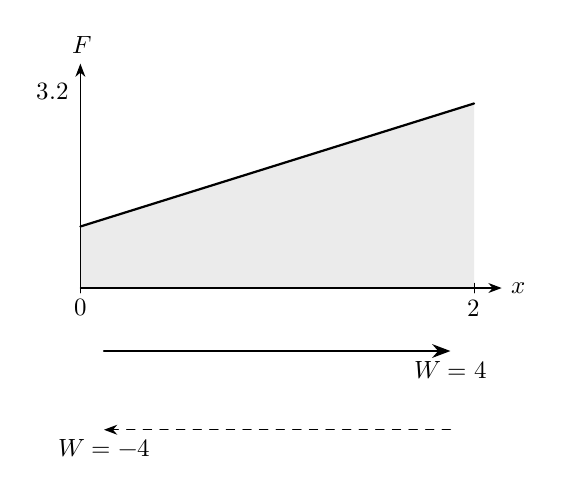
\begin{tikzpicture}[>=Stealth,font=\small,line cap=round,line join=round]
\draw[->,thin] (0,0.0) -- (5.35,0.0) node[right] {$x$};
\draw[->,thin] (0.0,0) -- (0.0,2.85) node[above] {$F$};
\draw[thick] plot coordinates {(0.00000,0.78125) (0.03125,0.79102) (0.06250,0.80078) (0.09375,0.81055) (0.12500,0.82031) (0.15625,0.83008) (0.18750,0.83984) (0.21875,0.84961) (0.25000,0.85938) (0.28125,0.86914) (0.31250,0.87891) (0.34375,0.88867) (0.37500,0.89844) (0.40625,0.90820) (0.43750,0.91797) (0.46875,0.92773) (0.50000,0.93750) (0.53125,0.94727) (0.56250,0.95703) (0.59375,0.96680) (0.62500,0.97656) (0.65625,0.98633) (0.68750,0.99609) (0.71875,1.00586) (0.75000,1.01562) (0.78125,1.02539) (0.81250,1.03516) (0.84375,1.04492) (0.87500,1.05469) (0.90625,1.06445) (0.93750,1.07422) (0.96875,1.08398) (1.00000,1.09375) (1.03125,1.10352) (1.06250,1.11328) (1.09375,1.12305) (1.12500,1.13281) (1.15625,1.14258) (1.18750,1.15234) (1.21875,1.16211) (1.25000,1.17188) (1.28125,1.18164) (1.31250,1.19141) (1.34375,1.20117) (1.37500,1.21094) (1.40625,1.22070) (1.43750,1.23047) (1.46875,1.24023) (1.50000,1.25000) (1.53125,1.25977) (1.56250,1.26953) (1.59375,1.27930) (1.62500,1.28906) (1.65625,1.29883) (1.68750,1.30859) (1.71875,1.31836) (1.75000,1.32812) (1.78125,1.33789) (1.81250,1.34766) (1.84375,1.35742) (1.87500,1.36719) (1.90625,1.37695) (1.93750,1.38672) (1.96875,1.39648) (2.00000,1.40625) (2.03125,1.41602) (2.06250,1.42578) (2.09375,1.43555) (2.12500,1.44531) (2.15625,1.45508) (2.18750,1.46484) (2.21875,1.47461) (2.25000,1.48438) (2.28125,1.49414) (2.31250,1.50391) (2.34375,1.51367) (2.37500,1.52344) (2.40625,1.53320) (2.43750,1.54297) (2.46875,1.55273) (2.50000,1.56250) (2.53125,1.57227) (2.56250,1.58203) (2.59375,1.59180) (2.62500,1.60156) (2.65625,1.61133) (2.68750,1.62109) (2.71875,1.63086) (2.75000,1.64062) (2.78125,1.65039) (2.81250,1.66016) (2.84375,1.66992) (2.87500,1.67969) (2.90625,1.68945) (2.93750,1.69922) (2.96875,1.70898) (3.00000,1.71875) (3.03125,1.72852) (3.06250,1.73828) (3.09375,1.74805) (3.12500,1.75781) (3.15625,1.76758) (3.18750,1.77734) (3.21875,1.78711) (3.25000,1.79687) (3.28125,1.80664) (3.31250,1.81641) (3.34375,1.82617) (3.37500,1.83594) (3.40625,1.84570) (3.43750,1.85547) (3.46875,1.86523) (3.50000,1.87500) (3.53125,1.88477) (3.56250,1.89453) (3.59375,1.90430) (3.62500,1.91406) (3.65625,1.92383) (3.68750,1.93359) (3.71875,1.94336) (3.75000,1.95312) (3.78125,1.96289) (3.81250,1.97266) (3.84375,1.98242) (3.87500,1.99219) (3.90625,2.00195) (3.93750,2.01172) (3.96875,2.02148) (4.00000,2.03125) (4.03125,2.04102) (4.06250,2.05078) (4.09375,2.06055) (4.12500,2.07031) (4.15625,2.08008) (4.18750,2.08984) (4.21875,2.09961) (4.25000,2.10938) (4.28125,2.11914) (4.31250,2.12891) (4.34375,2.13867) (4.37500,2.14844) (4.40625,2.15820) (4.43750,2.16797) (4.46875,2.17773) (4.50000,2.18750) (4.53125,2.19727) (4.56250,2.20703) (4.59375,2.21680) (4.62500,2.22656) (4.65625,2.23633) (4.68750,2.24609) (4.71875,2.25586) (4.75000,2.26562) (4.78125,2.27539) (4.81250,2.28516) (4.84375,2.29492) (4.87500,2.30469) (4.90625,2.31445) (4.93750,2.32422) (4.96875,2.33398) (5.00000,2.34375)};
\fill[black,opacity=.08] (0.0000,0.7812) -- (0.0625,0.8008) -- (0.1250,0.8203) -- (0.1875,0.8398) -- (0.2500,0.8594) -- (0.3125,0.8789) -- (0.3750,0.8984) -- (0.4375,0.9180) -- (0.5000,0.9375) -- (0.5625,0.9570) -- (0.6250,0.9766) -- (0.6875,0.9961) -- (0.7500,1.0156) -- (0.8125,1.0352) -- (0.8750,1.0547) -- (0.9375,1.0742) -- (1.0000,1.0938) -- (1.0625,1.1133) -- (1.1250,1.1328) -- (1.1875,1.1523) -- (1.2500,1.1719) -- (1.3125,1.1914) -- (1.3750,1.2109) -- (1.4375,1.2305) -- (1.5000,1.2500) -- (1.5625,1.2695) -- (1.6250,1.2891) -- (1.6875,1.3086) -- (1.7500,1.3281) -- (1.8125,1.3477) -- (1.8750,1.3672) -- (1.9375,1.3867) -- (2.0000,1.4062) -- (2.0625,1.4258) -- (2.1250,1.4453) -- (2.1875,1.4648) -- (2.2500,1.4844) -- (2.3125,1.5039) -- (2.3750,1.5234) -- (2.4375,1.5430) -- (2.5000,1.5625) -- (2.5625,1.5820) -- (2.6250,1.6016) -- (2.6875,1.6211) -- (2.7500,1.6406) -- (2.8125,1.6602) -- (2.8750,1.6797) -- (2.9375,1.6992) -- (3.0000,1.7188) -- (3.0625,1.7383) -- (3.1250,1.7578) -- (3.1875,1.7773) -- (3.2500,1.7969) -- (3.3125,1.8164) -- (3.3750,1.8359) -- (3.4375,1.8555) -- (3.5000,1.8750) -- (3.5625,1.8945) -- (3.6250,1.9141) -- (3.6875,1.9336) -- (3.7500,1.9531) -- (3.8125,1.9727) -- (3.8750,1.9922) -- (3.9375,2.0117) -- (4.0000,2.0312) -- (4.0625,2.0508) -- (4.1250,2.0703) -- (4.1875,2.0898) -- (4.2500,2.1094) -- (4.3125,2.1289) -- (4.3750,2.1484) -- (4.4375,2.1680) -- (4.5000,2.1875) -- (4.5625,2.2070) -- (4.6250,2.2266) -- (4.6875,2.2461) -- (4.7500,2.2656) -- (4.8125,2.2852) -- (4.8750,2.3047) -- (4.9375,2.3242) -- (5.0000,2.3438) -- (5.0000,0.0000) -- (0.0000,0.0000) -- cycle;
\draw[] (0.0,-0.06) -- (0.0,0.06);
\node at (0.0,-0.25) {$0$};
\draw[] (5.0,-0.06) -- (5.0,0.06);
\node at (5.0,-0.25) {$2$};
\node at (-0.35,2.5) {$3.2$};
\draw[->,thick] (0.3,-0.8) -- (4.7,-0.8) node[below] {$W=4$};
\draw[->,thin,dashed] (4.7,-1.8) -- (0.3,-1.8) node[below] {$W=-4$};

\end{tikzpicture}
\end{document}
